%% what_is_compgen.tex
%% Author: Leighton Pritchard
%% Copyright: James Hutton Institute
%% Introductory slides: What is Comparative Genomics?

% SUBSECTION
% What is Comparative Genomics?
\subsection{What is Comparative Genomics?}



%
\begin{frame}
  \frametitle{What Is Comparative Genomics?}
  Comparative genomics is$\ldots$ \\
  \Large{
    \textcolor{olive}{
      \textbf{
      The combination of genomic data, and comparative and evolutionary biology, to address questions of   genome structure, evolution, and function.
      }
    }
  }
\end{frame}

%
\begin{frame}
  \frametitle{Evolution is the central concept}
  \begin{center}
    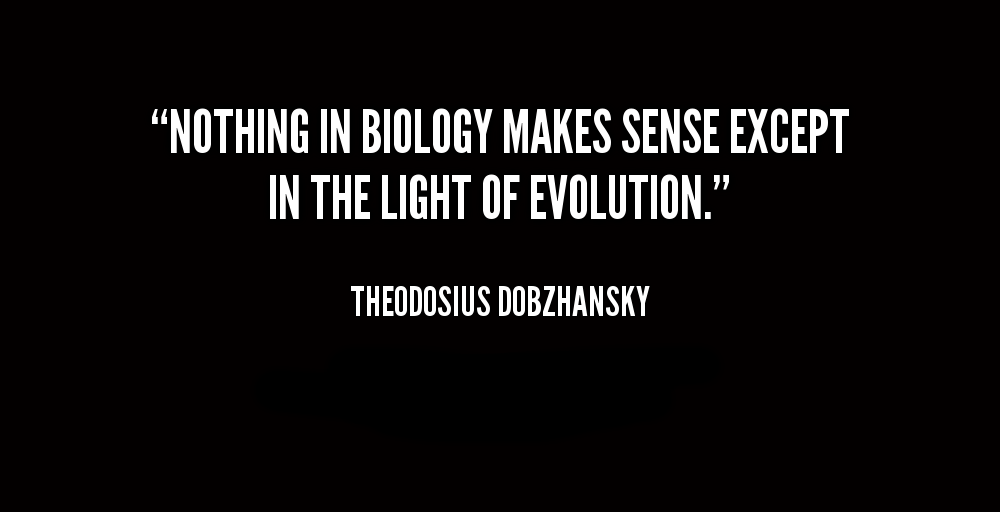
\includegraphics[width=\textwidth]{images/dobzhansky_quote}
  \end{center}  
\end{frame}

%
\begin{frame}
  \frametitle{Comparison of physical features}
  How do we determine that features are related, and evolved? \\
  \begin{center}
    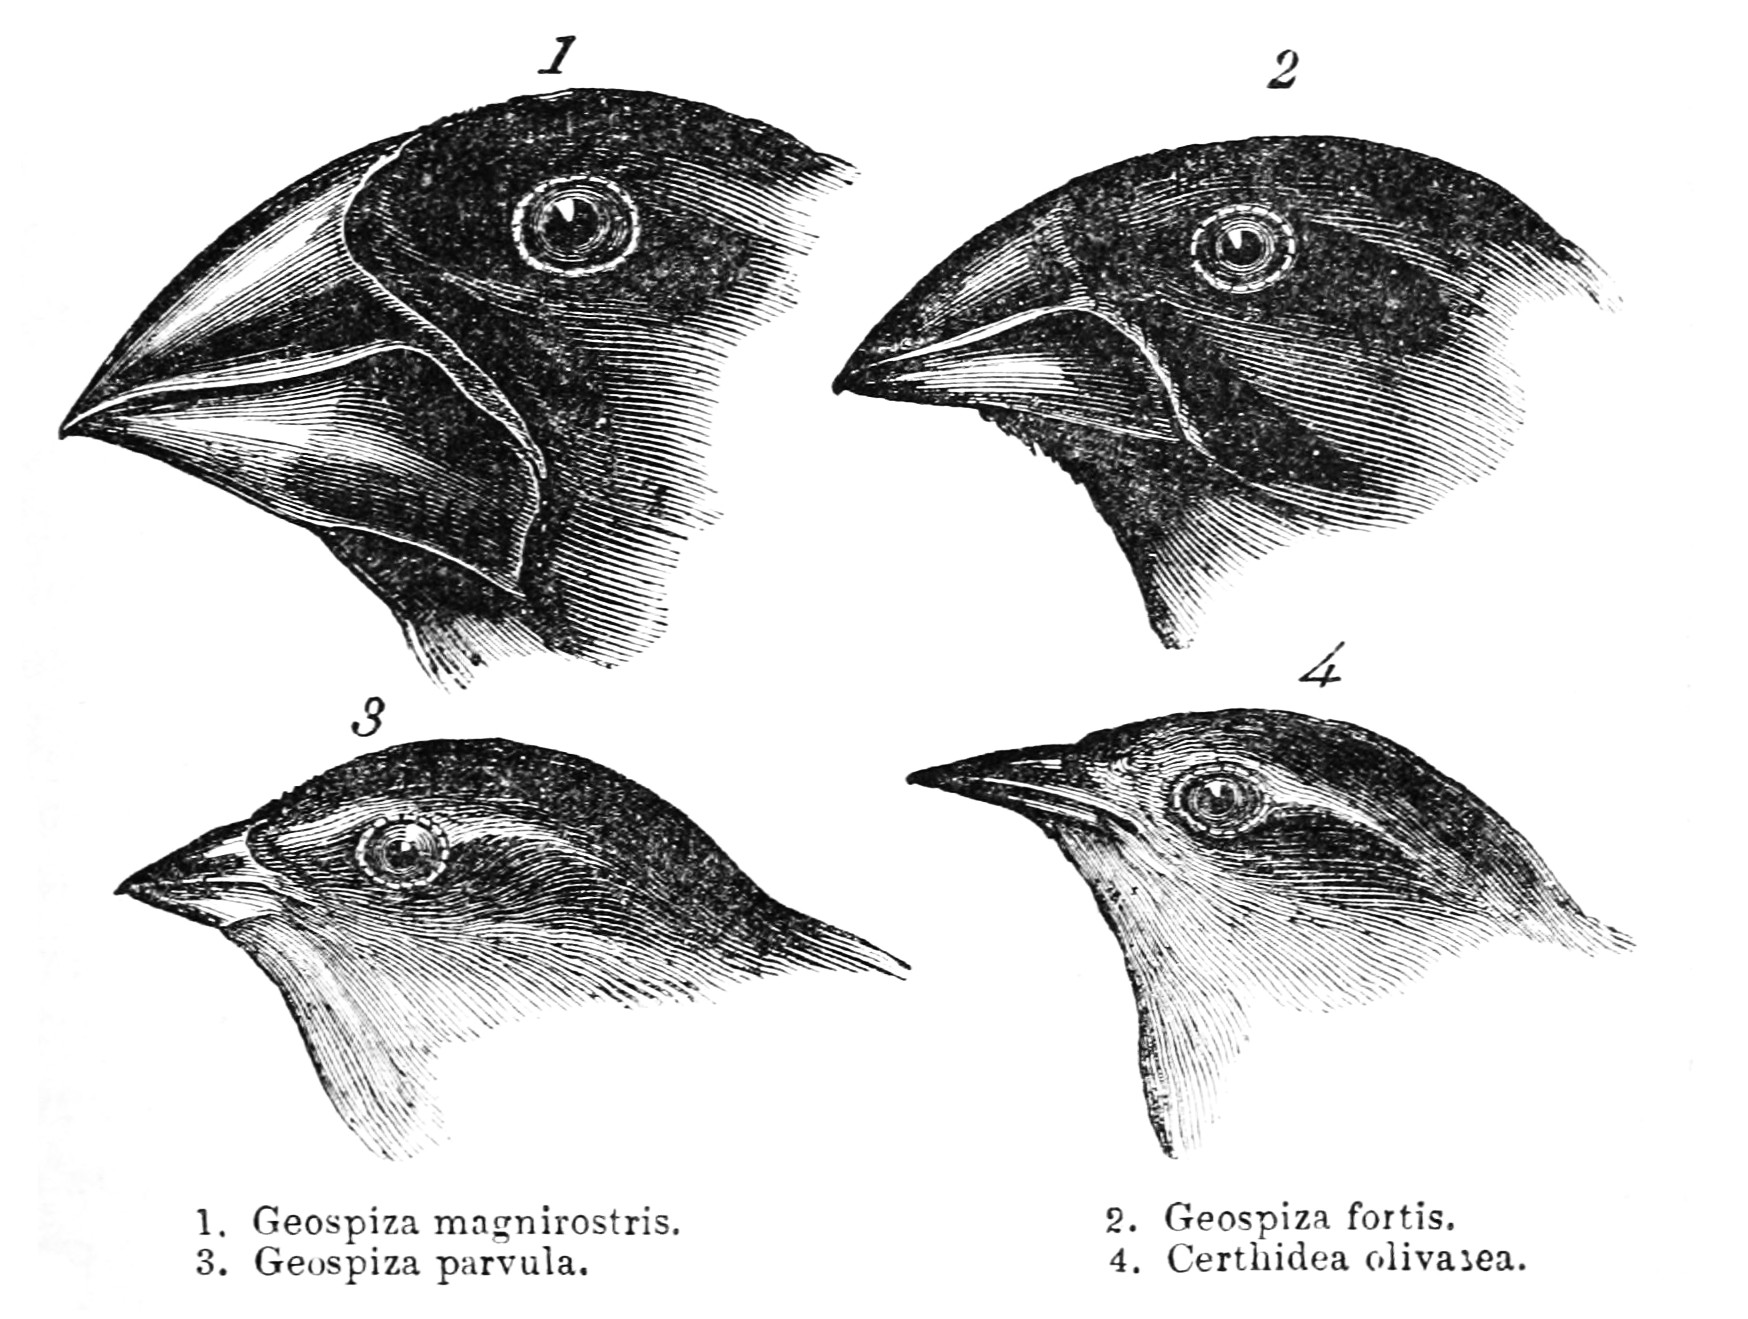
\includegraphics[width=0.8\textwidth]{images/darwin_finches}
  \end{center}  
\end{frame}

%
\begin{frame}
  \frametitle{Comparison of sequence features}
  Multiple alignment of ATP synthase \\
  \begin{center}
    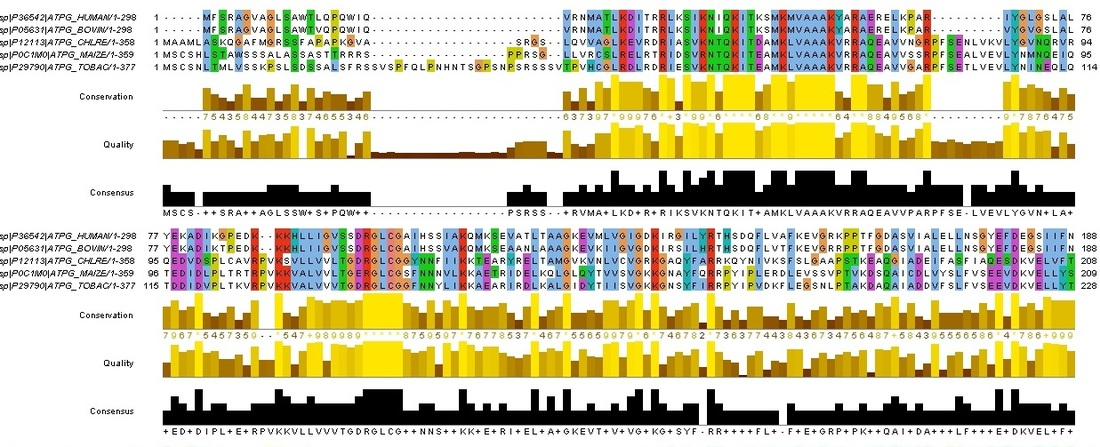
\includegraphics[width=\textwidth]{images/atp_synthase_alignment}
  \end{center}  
\end{frame}

%
\begin{frame}
  \frametitle{Comparison of genome features}
  Sequence similarity of individual features \\
  \begin{center}
    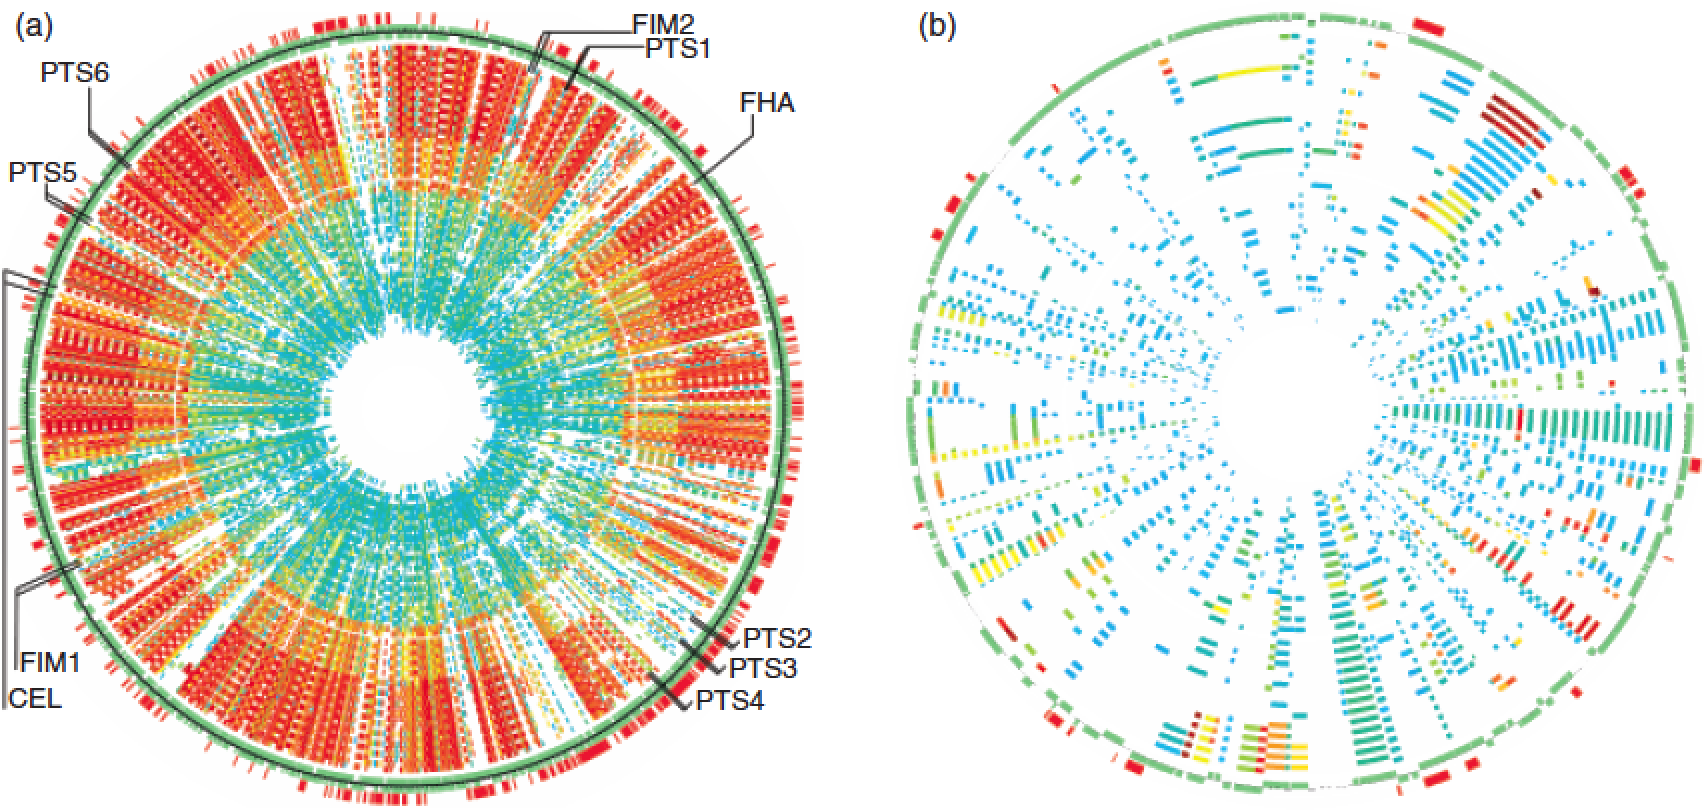
\includegraphics[width=\textwidth]{images/salmonella_circular_comparison}
  \end{center}  
\end{frame}

%
\begin{frame}
  \frametitle{Comparison of genome features}
  Genome structural rearrangements \\
  \begin{center}
    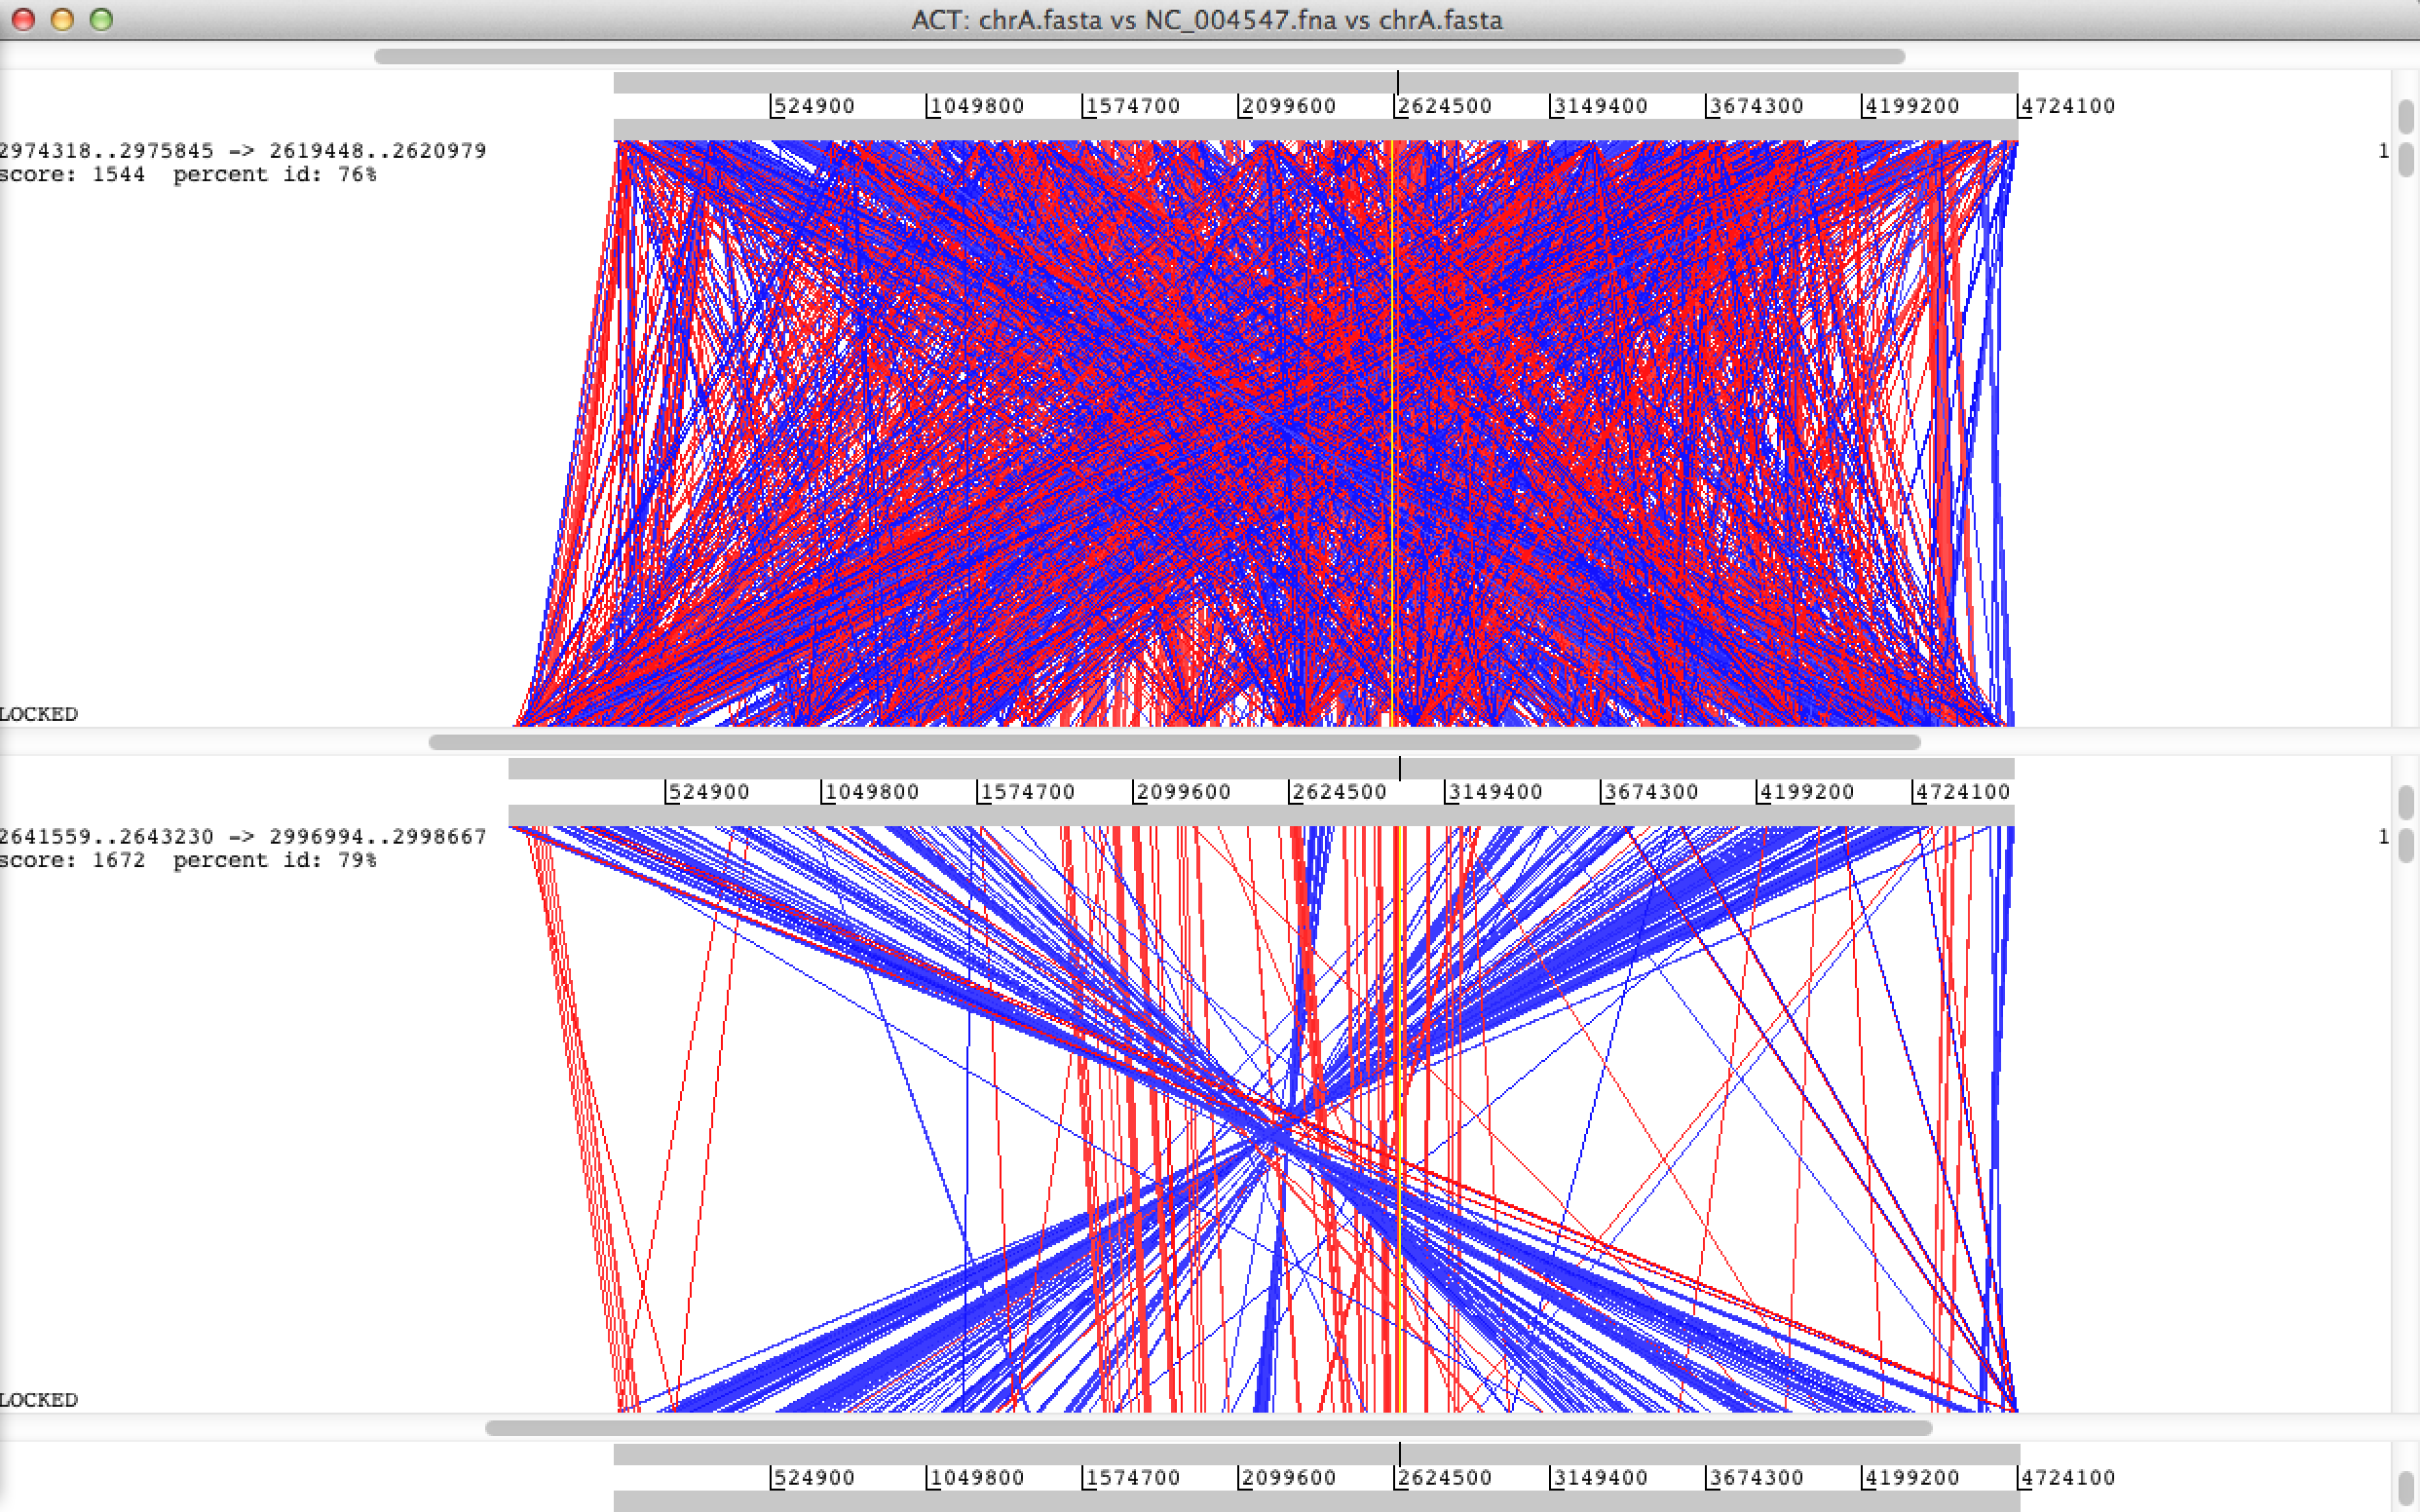
\includegraphics[width=\textwidth]{images/act_rearrangement}
  \end{center}  
\end{frame}

%
\begin{frame}
  \frametitle{Why comparative genomics?}
    \begin{columns}[c] 
      \column{.6\textwidth} 
        \begin{itemize}
         \item \textcolor{hutton_green}{Genomes describe heritable characteristics}
         \item Related organisms share ancestral genomes
         \item \textcolor{hutton_blue}{Functional elements encoded in genomes are common to related organisms}
        \end{itemize}
      \column{.4\textwidth}
        
\includegraphics[width=\textwidth]{images/darwin_tree}
    \end{columns}  
\end{frame}

%
\begin{frame}
  \frametitle{Why comparative genomics?}
    \begin{columns}[c] 
      \column{.6\textwidth} 
        \begin{itemize}
         \item \textcolor{RawSienna}{Transfer of functional understanding from model systems (\textit{E. coli}, \textit{A. thaliana}, \textit{D. melanogaster}) to non-model systems}
         \item \textcolor{olive}{Genome comparisons can be informative, even for distantly-related organisms}
        \end{itemize}
      \column{.4\textwidth}
        
\includegraphics[width=\textwidth]{images/darwin_tree}
    \end{columns}  
\end{frame}

%
\begin{frame}
  \frametitle{Genomes are informative, but$\ldots$}
  \textcolor{hutton_blue}{\textbf{CONTEXT:}} epigenetics, tissue differentiation, mesoscale systems, etc.\\
  \begin{center}  
    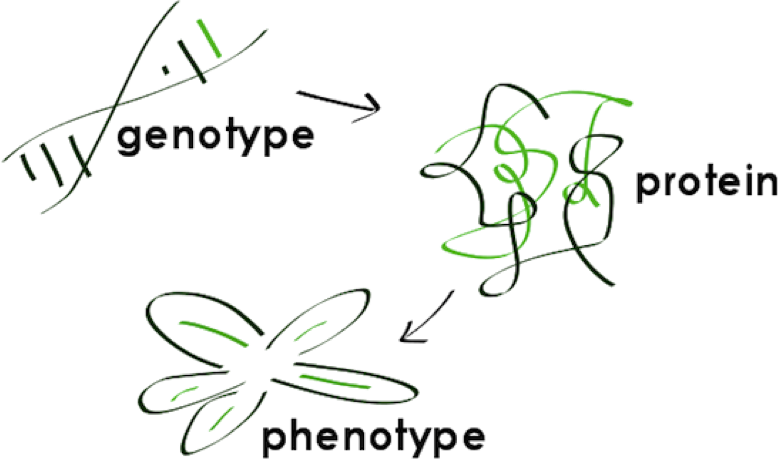
\includegraphics[width=0.7\textwidth]{images/genotype_protein_phenotype}
  \end{center}    
  \textcolor{hutton_green}{\textbf{PHENOTYPIC PLASTICITY:}} responses to temperature, stress, environment, etc.
\end{frame}

%
\begin{frame}
  \frametitle{Genomes to systems}
    \begin{columns}[c] 
      \column{.6\textwidth} 
        \textcolor{RawSienna}{\textbf{Functional Genomics}}
        \begin{itemize}
         \item \textcolor{hutton_green}{Genomic differences can underpin phenotypic (morphological or physiological) differences.}
         \item Where phenotypes/other organism-level properties are known, comparison of genomes can give mechanistic or functional insight into differences (e.g. GWAS).
         \item \textcolor{hutton_blue}{Genomic changes reveal evolutionary processes and constraints.}
        \end{itemize}
      \column{.4\textwidth}
        
\includegraphics[width=\textwidth]{images/darwin_tree}
    \end{columns}  
\end{frame}



